\documentclass{scrartcl}
\usepackage[utf8]{inputenc}
\usepackage{graphicx}
\usepackage{listings}
\usepackage{hyperref}

\begin{document}

\section{Introduction}
Linux Installation: Ich denke Ihr wisst wie euer System funktioniert.

\subsection{Systemcheck}
% Windows 64 bit / 32 bit -> in system nach schauen
Als erstes ist wichtig zu wissen, ob dein Computer über eine 64-bit oder 32-bit Architektur verfügt. Navigiere dazu zu "Dieser PC", rechtsklicke und wähle Eigenschaften.

\begin{center}
    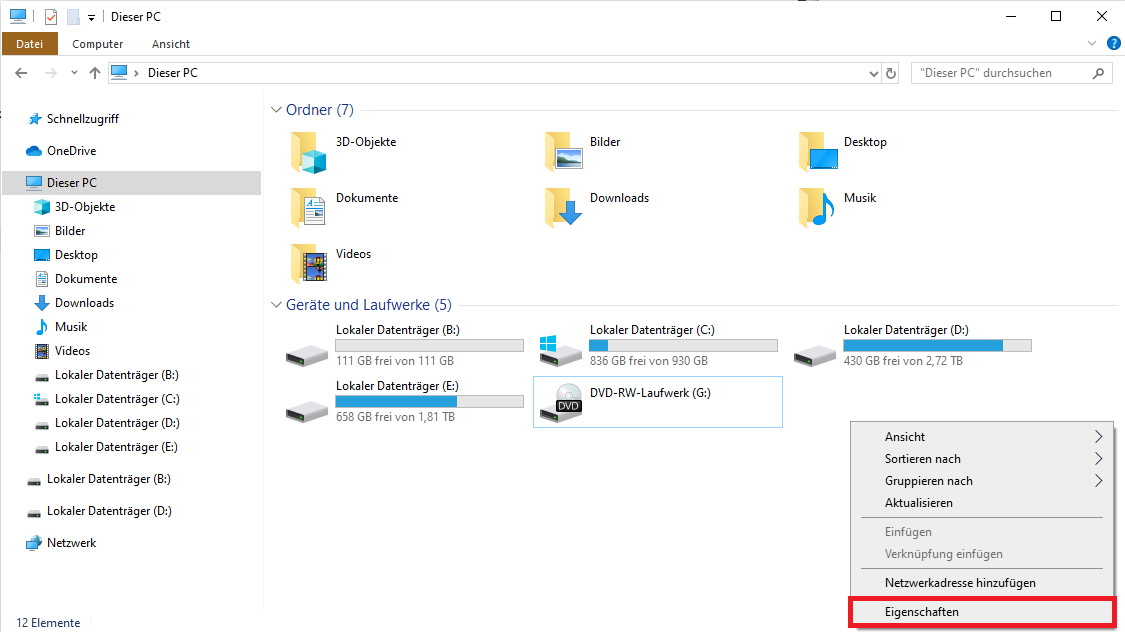
\includegraphics[width=.9\textwidth]{Screenshot_1.png}
\end{center}
    
Im nun geöffneten Fenster kannst du unter Systemtyp nachsehen, ob du über eine 64-bit oder 32-bit Architektur verfügst.\\
\begin{center}
    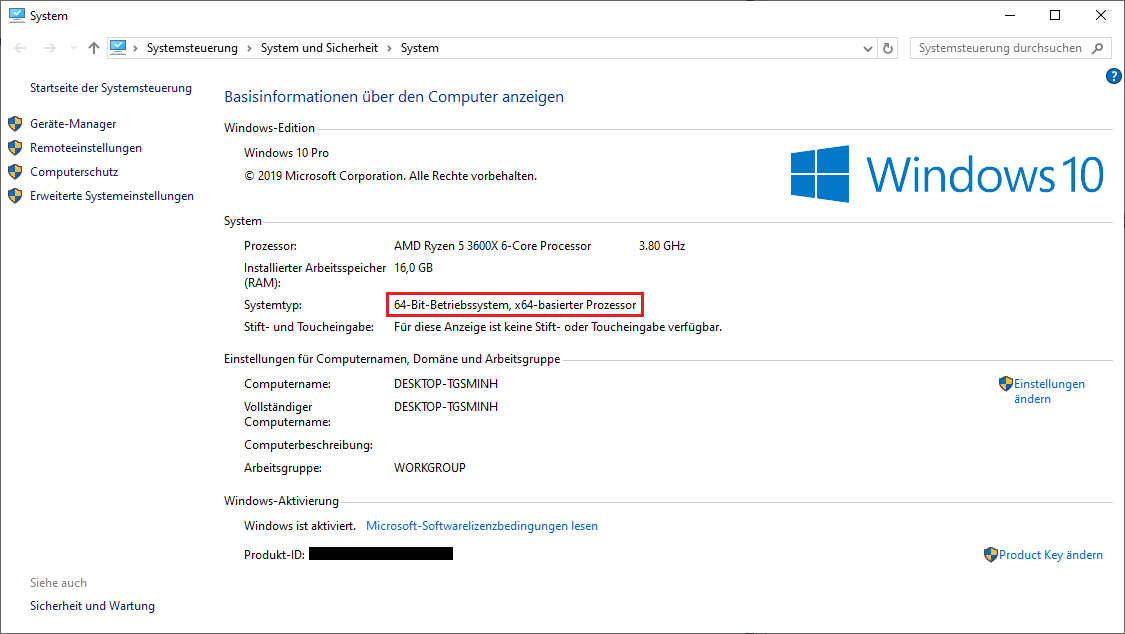
\includegraphics[width=.9\textwidth]{Screenshot_2.png}
\end{center}
% Umgebungsvariablen setzen -> PATH (vielleicht)
% Eclipse Install

\section{Installation}
\subsection{Java JDK}
Lade eine Passende Java-Version herunter. Gehe dazu auf \url{https://adoptopenjdk.net/} Wähle OpenJDK14
aus und drücke auf "Neueste Veröffentlichung".\\
\begin{center}
    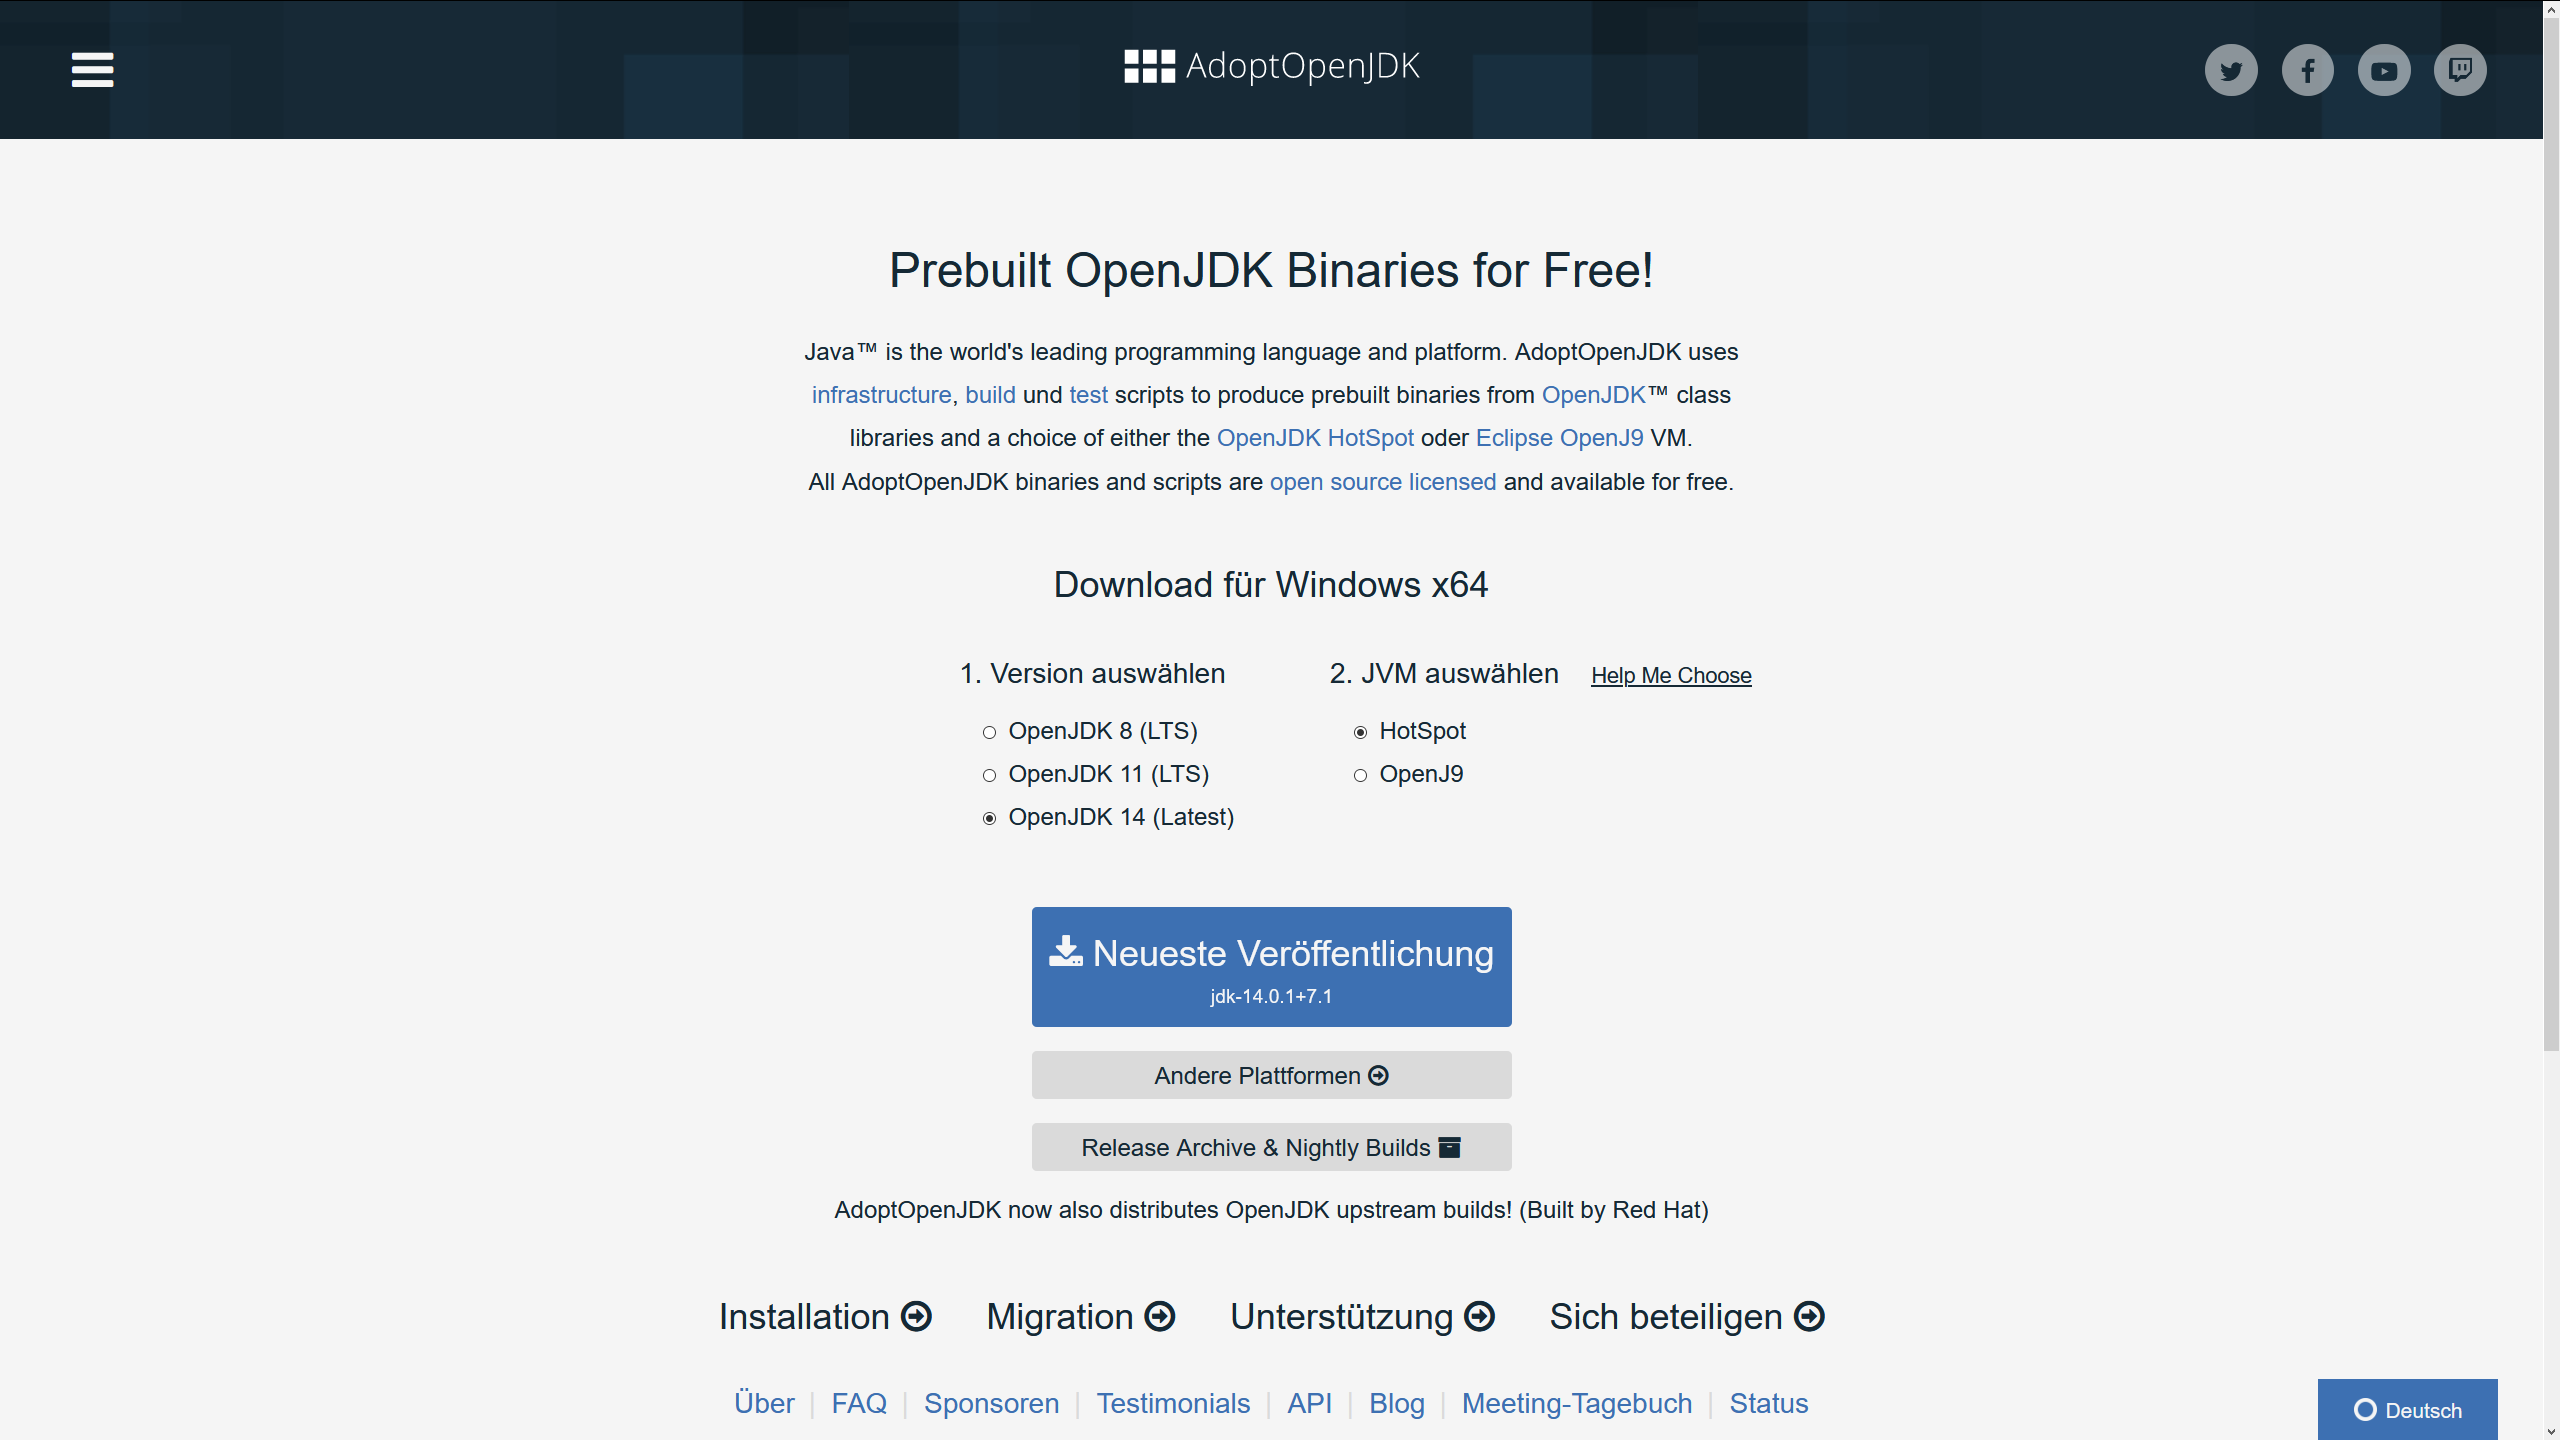
\includegraphics[width=.88\textwidth]{Screenshot_6.png}
\end{center}
Führe die .msi Datei aus und Folge den Installationsanweisungen.\\
Nun folgt die Installation von Eclipse.
Wenn du über eine 64-Bit Architektur verfügst gehe zunächst auf https://www.eclipse.org/downloads/. Dann drücke den Download-Button.
%\includegraphics[width=\textwidth]{Screenshot_2.2.png}
Für die 32-Bit Version gehe auf https://www.eclipse.org/downloads/packages/release/2018-09/r und wähle Windows 32-Bit aus.\\

\begin{center}
    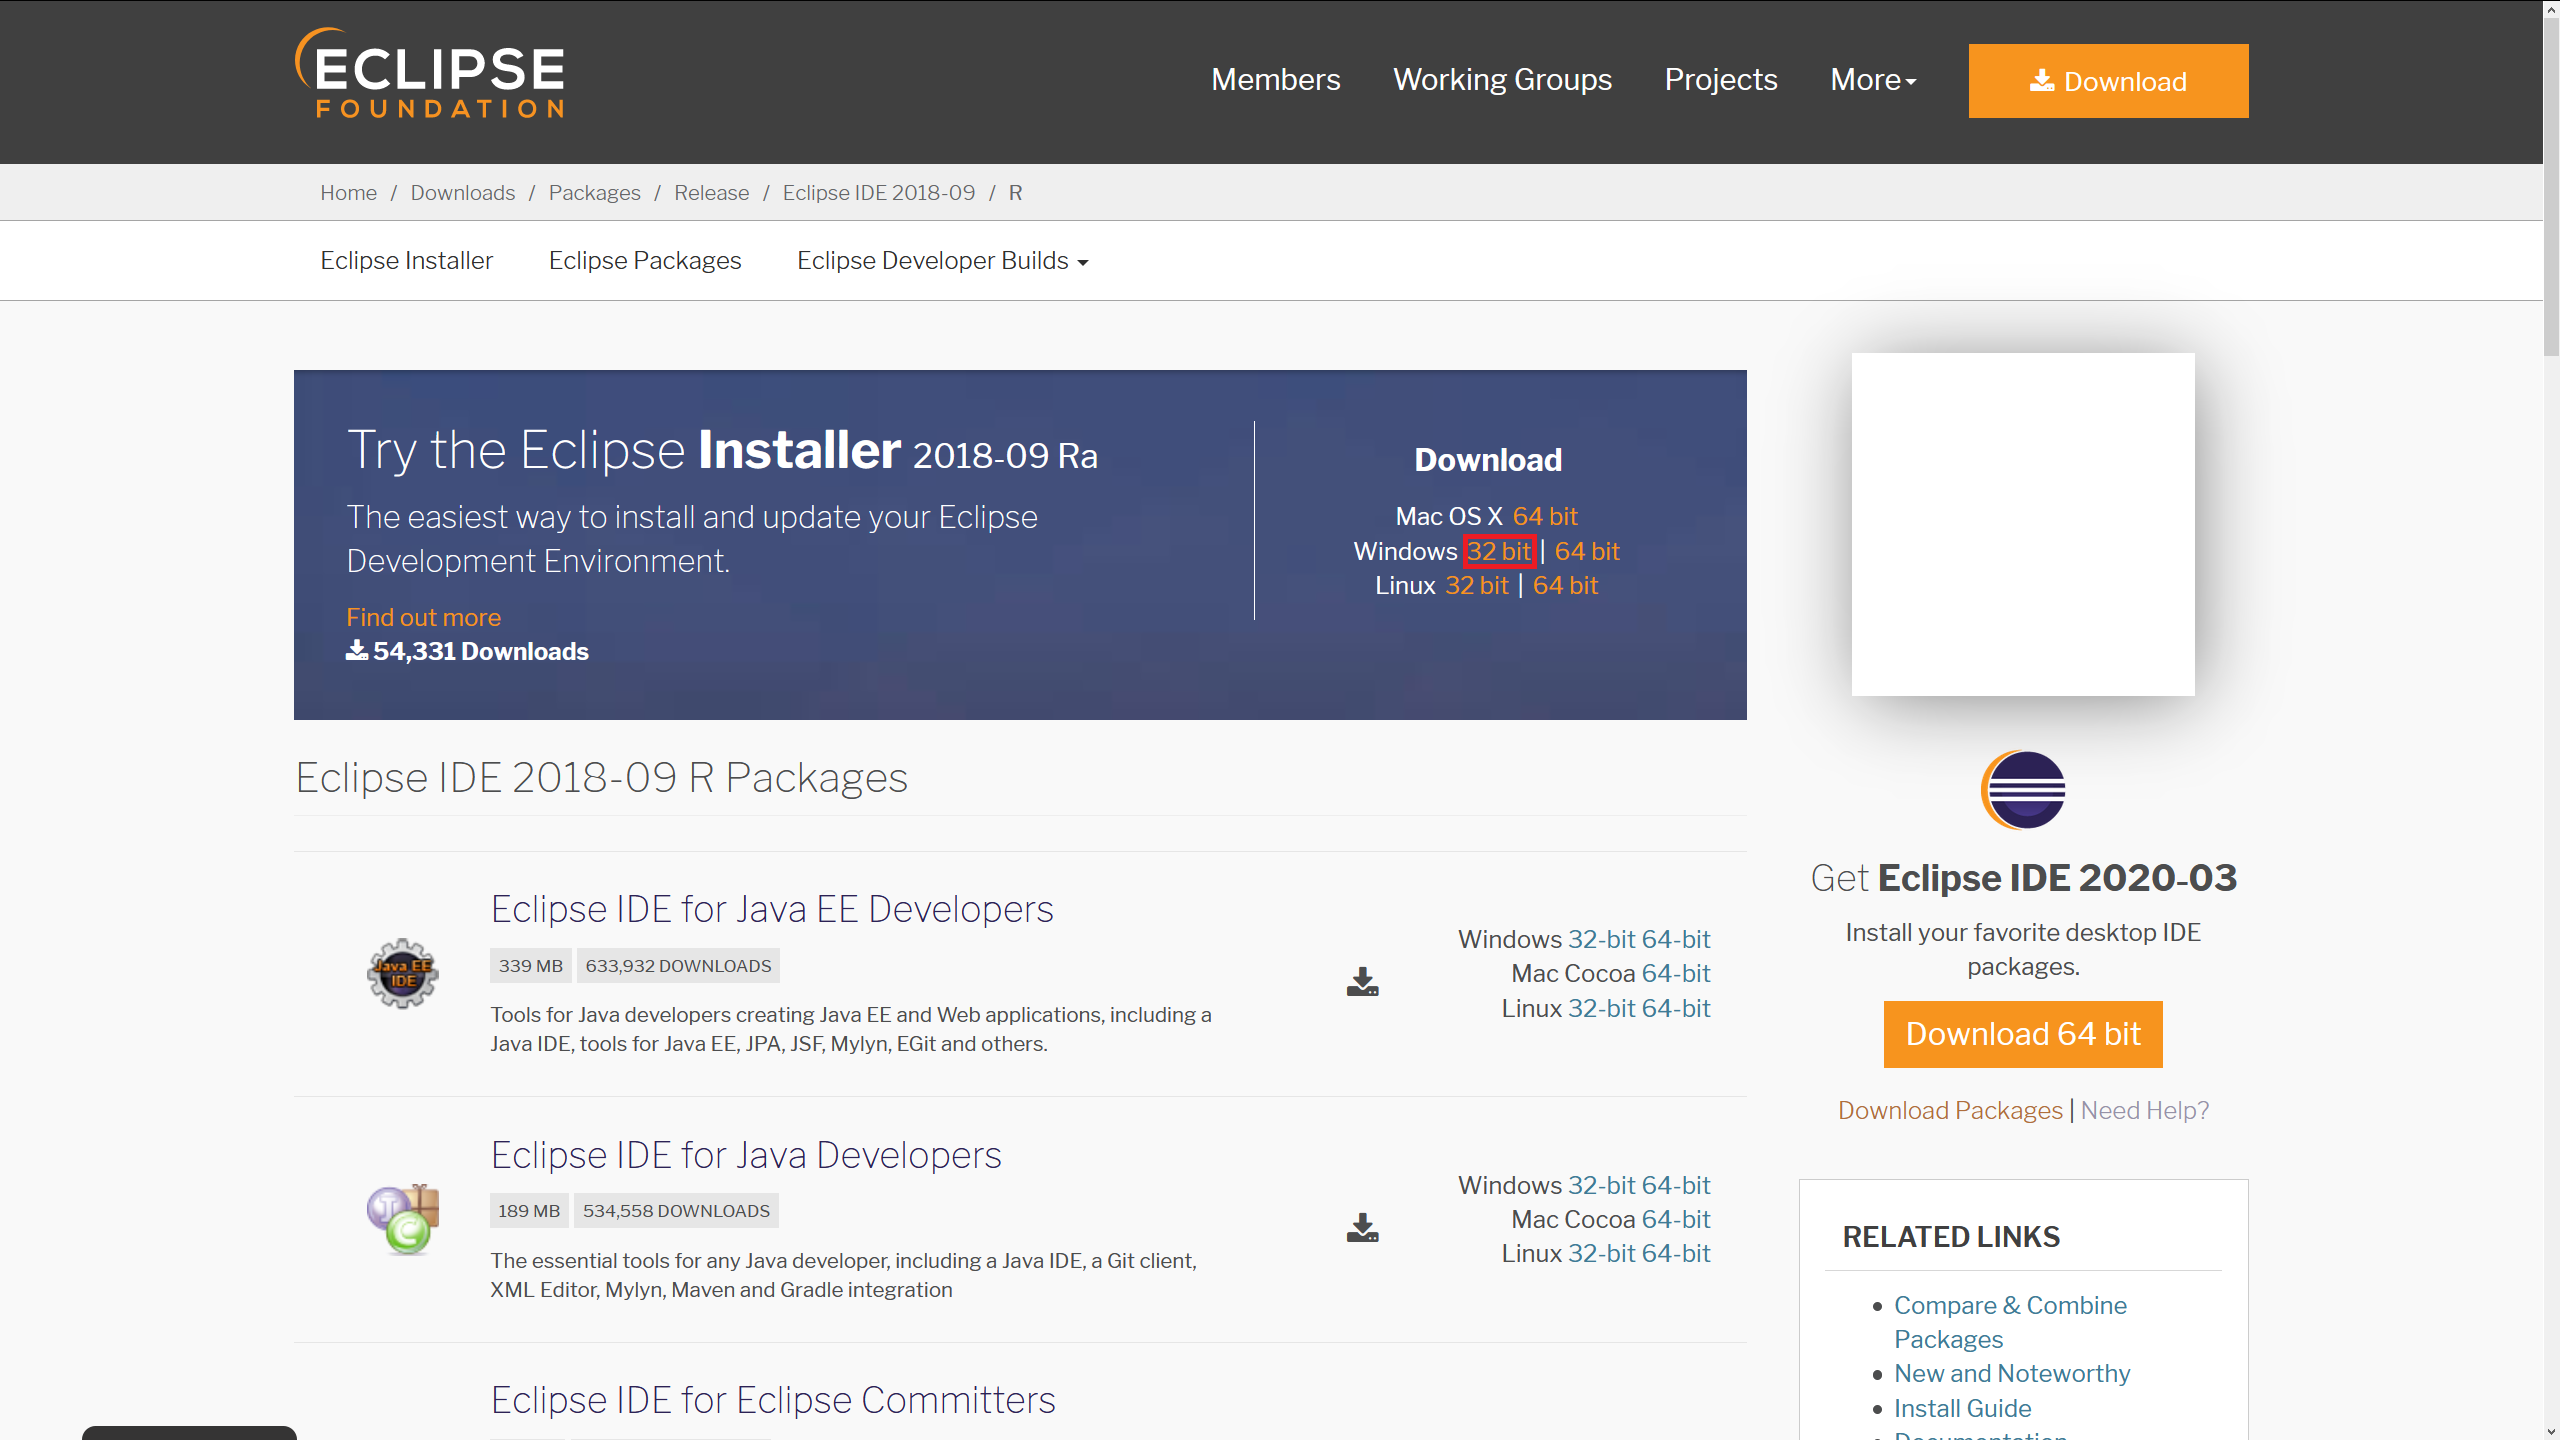
\includegraphics[width=.88\textwidth]{Screenshot_2.3.png}
\end{center}

\newpage
\subsection{Eclipse (IDE)}
Führe nun den Eclipse-Installer aus. Wähle die "Eclipse-IDE for Java Developers".\\
\begin{center}
    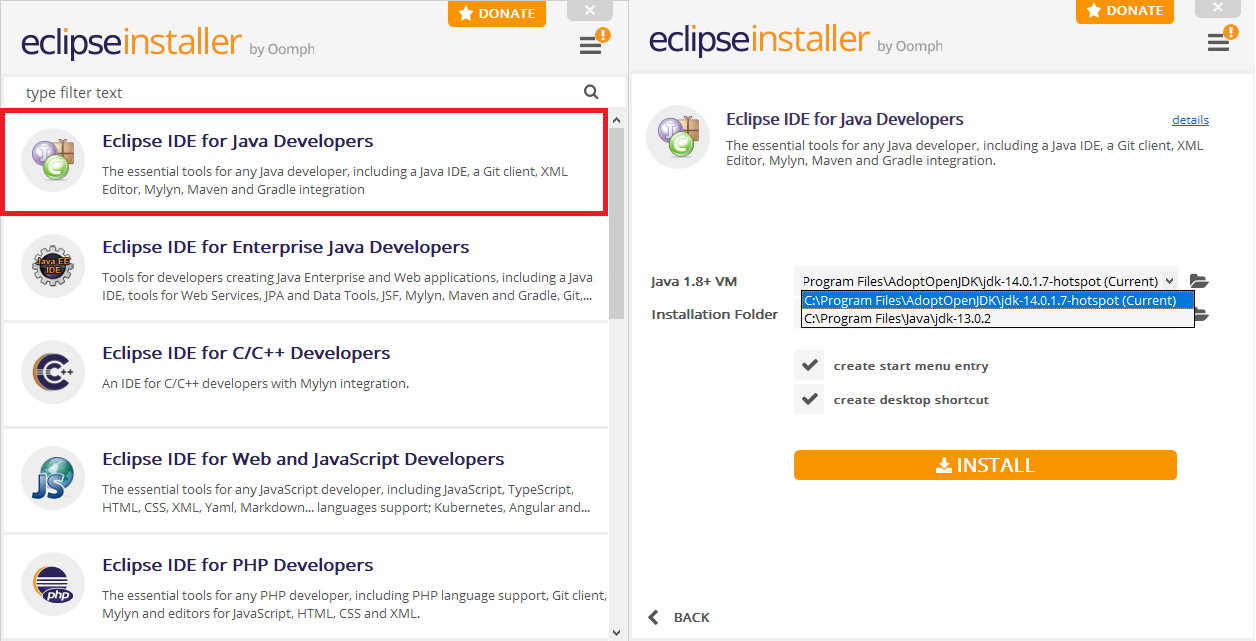
\includegraphics[width=\textwidth]{Screenshot_7.png}
\end{center}
Wähle als "Java 1.8+ VM" jdk-14 und drücke auf Install\\
\subsection{Importieren}
Um ein Projekt zu importieren, gehe zu File $\rightarrow$ Import $\rightarrow$ Maven  $\rightarrow$ Existing Maven Project  $\rightarrow$  Browse, wähle das zu Importierende Projekt aus und drücke anschließend Finish. Achte darauf, dass das Projekt unkomprimiert, also nicht als .zip oder .rar Datei, vorliegt.\\





% TODO (maybe) Grobe Übersicht wichtiger UI Elemente 
\section{Anmerkungen}
Optional: Um die Integrität des Downloads zu überprüfen und sicher zu stellen das eine unveränderte Version von der Datei heruntergeladen wurde, wie es der Herausgeber angibt, kann man den angebebenen SHA auf der Download Seite mit dem SHA der heruntergeladenen Datei vergleichen. In dem Ordner in welchem die Datei liegt, halte shift gedrückt und rechtsklicke um das Kontextmenü zu öffnen. Wähle "Powershell Fenster hier öffnen aus". Gebe den Befehl 
% TODO CODE
    \begin{lstlisting}
    Get-FileHash <Filename> -Algorithm SHA512 | Format-List 
    \end{lstlisting}

% ende todo
ein und ersetze $<$Filename$>$ durch den Namen der heruntergeladenen Datei.

\end{document}
